%
% fig-parallelogramm.tex
%
% (c) 2025 Prof Dr Andreas Müller
%
\begin{figure}
\centering
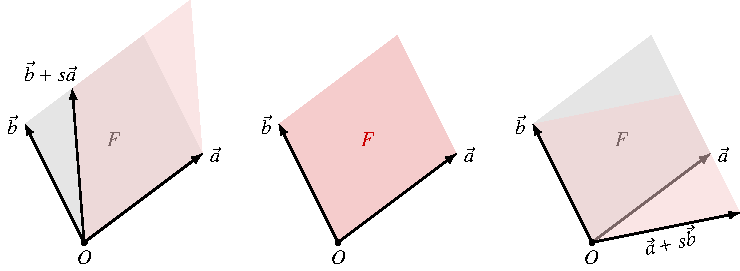
\includegraphics{chapters/040-green/images/parallelogramm.pdf}
\caption{Die Parallelogrammfläche ist eine bilineare Funktion der
Kantenvektoren.
Sie ändert nicht, wenn man einen Kantenvektor
um ein Vielfaches des anderen ändert.
Dies ist die gemeinsame Eigenschaft vieler physikalischer Grössen,
die gemeinhin mit dem Vektorprodukt modelliert werden.
\label{buch:green:2vektoren:fig:parallelogramm}}
\end{figure}
